%% 
%% Copyright 2007-2019 Elsevier Ltd
%% 
%% This file is part of the 'Elsarticle Bundle'.
%% ---------------------------------------------
%% 
%% It may be distributed under the conditions of the LaTeX Project Public
%% License, either version 1.2 of this license or (at your option) any
%% later version.  The latest version of this license is in
%%    http://www.latex-project.org/lppl.txt
%% and version 1.2 or later is part of all distributions of LaTeX
%% version 1999/12/01 or later.
%% 
%% The list of all files belonging to the 'Elsarticle Bundle' is
%% given in the file `manifest.txt'.
%% 
%% Template article for Elsevier's document class `elsarticle'
%% with harvard style bibliographic references

\documentclass[preprint,12pt,authoryear]{elsarticle}

%Please do not delete this section
\makeatletter
\def\ps@pprintTitle{%
 \let\@oddhead\@empty
 \let\@evenhead\@empty
 \def\@oddfoot{\centerline{}}%
 \let\@evenfoot\@oddfoot}
\makeatother

%% For including figures, graphicx.sty has been loaded in
%% elsarticle.cls. If you prefer to use the old commands
%% please give \usepackage{epsfig}

%% The amssymb package provides various useful mathematical symbols
\usepackage{amssymb}
%% The amsthm package provides extended theorem environments
%% \usepackage{amsthm}

\usepackage{hyperref}
\usepackage{multirow}
\usepackage{mathptmx}
\usepackage{array}
\usepackage{amsmath}
\usepackage[margin=2.5cm]{geometry}
\newcounter{metric}
\renewcommand{\themetric}{2.3.\arabic{metric}} % format the number however you like
\usepackage{caption}
\captionsetup{font=small}
\usepackage{float}
\usepackage{subcaption}

\journal{24th International Working Seminar on Production Economics}

\begin{document}
\begin{frontmatter}

\title{extending Lean to Non-Manufacturing Workflows in Semiconductor Supply Chains}

\author[label1,label2,label3]{Niklas Lauter}
    \address[label1]{Dept.\ of Production Management, University of Economics, 1020 Vienna, Austria\\
    \href{mailto:gerald.reiner@wu.ac.at}{gerald.reiner@wu.ac.at}\\
    }
    
\author[label2]{Silvia Casati}

\author[label2]{Sara Giusiano}

\author[label2]{Christine O'Brien}

\author[label2]{Hans Ehm}
    \address[label2]{Supply Chain Innovation, Infineon Technologies AG, 85579 Neubiberg, Germany\\
    \href{mailto:Niklas.Lauter@infineon.com}{niklas.lauter@infineon.com}\\
    \href{mailto:Silvia.Casati@infineon.com}{silvia.casati@infineon.com}\\
    \href{mailto:Sara.Giusiano@infineon.com}{sara.giusiano@infineon.com}\\
    \href{mailto:Christine.OBrien@infineon.com}{christine.obrien@infineon.com}\\
    \href{mailto:Hans.Ehm@infineon.com}{hans.ehm@infineon.com}\\
    }
\author[label1]{Gerald Reiner}

%Please indicate the presenting author    
    \address[label3]{Presenting author}

\begin{abstract}
In todays industry 5.0 context, the global semiconductor supply chain integrates complex manufacturing systems with a comparably complex network of non-manufacturing workflows and human operations. Operating Curve (OC) principles, applied within Lean for Complex Flow Manufacturing Principles (LCFM), have proven effective for optimizing utilization (U) and speed with low variability, especially in recurrent manufacturing flows in fabs. This paper extends and applies the traditional OC framework to selective non-manufacturing workflows in global semiconductor supply chains. A quasi-experimental, field-based, pretest-posttest, multicase design pilot study was conducted, focusing on a baseline case and two intervention cases from non-manufacturing enabling processes. The study is positioned as intervention-based research (IBR): a plausible theory basket (factory-physics-based OC management) is deployed into practice through real process interventions, and the resulting surprises are used to recalibrate that theory. The processes were modeled using BPMN-based workflow representations and OWL ontologies to create a queryable semantic layer. Initial results are promising: the OC approach demonstrated for the chosen processes RPT and FF reduction. Additionally, new insights have been gained: while manufacturing faces very complex dynamics that cause variability, non-manufacturing human-in-the-loop workflows, despite often being less complex, exhibit governance-driven and cross-functional handoff volatility. These insights lay the groundwork for future research to determine whether such effects can be mitigated or whether human-centric adaptations of factory physics are needed in non-manufacturing domains. As supply chains grow in complexity, extending lean principles for complex flow manufacturing to non-manufacturing workflows opens overall end-to-end efficiency opportunities in one ``virtual fab'' semiconductor supply chain approach.

\end{abstract}

\begin{keyword}
    %% keywords here, in the form: keyword \sep keyword
    Lean Manufacturing \sep Semiconductor \sep Supply Chain \sep Efficiency.
\end{keyword}

\end{frontmatter}

%% main text
\section{Introduction}\label{sec:Introduction}

The semiconductor industry constitutes one of the most complex and capital-intensive production systems globally \citep{monch2013}. Its competitiveness is predicated not only on technological leadership but increasingly on the capacity to efficiently manage highly interconnected supply chains. Although semiconductor manufacturing systems have been systematically optimized over decades through the application of lean principles and factory physics, an increasing portion of value creation now arises from activities beyond the factory floor \citep{LauterEhmReiner2025}.

Semiconductor supply chains and workflows have transformed into globally distributed, digitally enabled networks that integrate advanced manufacturing operations with diverse non-manu\-facturing workflows \citep{Felsberger2022}. These workflows encompass activities such as new product sampling, fab-overarching process flows, and enabling processes. While they do not directly alter the physical characteristics of products, these workflows significantly influence the efficiency, effectiveness, and overall performance of the supply chain.

The application of Lean methodologies for Complex Flow Manufacturing (LCFM), with Operating Curve (OC) principles \citep{HackmanLeachman1989}, has proven highly efficient \citep{ehm2011, fayed2008} in semiconductor manufacturing for balancing throughput (TH), resource utilization (U), and process variability. Grounded in factory physics, these principles provide a quantitative framework for analyzing trade-offs between speed and efficiency in re-entrant, high-variability production environments \citep{monch2013} and for optimizing speed and efficiency simultaneously while reducing variability (alpha). Their demonstrated success has established OC management as a standard practice for performance optimization in semiconductor fabrication facilities worldwide.

Nevertheless, the applicability of these principles to non-manufacturing domains remains underexplored. Consequently, performance losses in non-manufacturing workflows often remain obscured and are rarely addressed by physics-based efficiency models.

This study addresses this research gap by extending the OC principles to selected non-manu\-facturing workflows within global semiconductor supply chains. Building upon previous conceptual work \citep{LauterEhmReiner2025}, we examine whether the explanatory and improvement potential of OC-based performance frameworks can be effectively transferred from manufacturing to non-manufacturing contexts. In this approach, non-manufacturing processes are conceptualized as flow systems that can be rigorously modeled, quantitatively measured, and systematically improved, rather than as inherently unstructured or solely qualitative activities.

Empirically, this study employs a quasi-experimental, field-based, pretest--posttest multi-case design. Selected non-manufacturing enabling processes are modeled utilizing BPMN-based workflow representations and analyzed using Flow Factor (FF) based performance metrics. Methodologically, the work is framed as intervention-based research (IBR) in the sense of \citet{oliva2019intervention} and \citet{chandrasekaran2020ibr}: the OC theory basket is applied through interventions, and the deviations between expected and observed outcomes are exploited as a source of new theory. The results demonstrate that the OC logic maintains explanatory power in non-manufacturing environments, particularly in flow efficiency, leveraging synchronization potentials, and identifying dominant sources of variability. Simultaneously, the findings underscore unique characteristics of human-in-the-loop workflows that complicate the direct, unmodified application of factory physics.

By extending LCFM principles to non-manufacturing workflows, this research advances a more integrated perspective on supply chain performance within the semiconductor industry. It supports the conceptualization of global semiconductor supply chains as a ``virtual fab'' \citep{ehm2011}, in which manufacturing and non-manufacturing processes are jointly optimized within an interconnected efficiency framework. The findings establish a basis for future research on human-centric adaptations of factory physics and the systematic management of non-manufacturing complexity in advanced industrial supply chains. BPMN-based process models are additionally formalized into a machine-readable semantic layer (OWL ontologies), which renders the measured RPT queryable and enables consistent cross-case Operating Curve benchmarking. The next chapters are grouped as follows: first, the relevance of lean for complex flow manufacturing is described; this is followed by the need for its application, the related research questions and methodology, the modeling and measurement apparatus, which includes the semantic-layer extension, the results achieved, and a discussion of the results and suggested follow-up research.

\subsection{The Relevance of Lean for Complex Flow Management in the Global Semiconductor Supply Chain}\label{sec:The Relevance of Lean for Complex Flow Management in the Global Semiconductor Supply Chain}

In manufacturing environments, lean management is used as a fundamental objective and has been central to semiconductor manufacturing for decades \citep{Liker2004}. 

Lean thinking seeks to maximize value by stabilizing the process flow and aligning resources with customer demand. In semiconductor fabrication facilities, these principles are systematically applied to balance speed, U, and process variability in highly capital-intensive, complex production settings \citep{Liker2004}.

In this context, the LCFM principles \citep{bauer2011LCFM} show that the 4 partners: machine, human, material, and method (4M) \citep{Schmielau2024} are used in the most efficient and effective way.

Efficiency refers to ``doing things right'', meaning in the best possible way, minimizing resources, time, and effort while maintaining quality \citep{Liker2004}, while effectiveness refers to ``doing the right things'', which refers to our supply chain connected to the achievement of the desired goals and the output that relates to customer requirements in terms of quality, quantity, and time \citep{Liker2004}.

From the perspective of lean for complex flow management, efficiency denotes the uninterrupted flow of work characterized by minimal waiting, rework, and overburden, whereas effectiveness ensures that organizational efforts are focused on the appropriate objectives at the optimal time %source.

As semiconductor supply chains have evolved into globally distributed, digitally interconnected systems, the applicability of lean principles has extended beyond manufacturing. An increasing proportion of variability and coordination challenges arises from non-manufacturing workflows as globalization and VUCA worlds are growing \citep{SchusterStork2021}. Although these processes do not directly consume production capacity, they substantially affect speed and cost in global supply chains \citep{hopp2001}.This digital transformation is the subject of the emerging Lean~4.0
perspective, which studies how digital technologies support and reinforce lean practices.\ \citet{cifone2021lean40} show that digital technologies
reduce non-value-adding work through eight mechanisms, grouped into two
categories:

\begin{itemize}
  \item{Augmenting operational execution}
        \begin{itemize}
          \item speed,
          \item precision,
          \item spatial flexibility, and
          \item temporal flexibility;
        \end{itemize}
  \item{Augmenting decision-making}
        \begin{itemize}
          \item visibility,
          \item feedback,
          \item engagement, and
          \item prevention.
        \end{itemize}
\end{itemize}
%
These mechanisms are particularly pertinent to non-manufacturing workflows,
where waste is predominantly informational, coordination-driven, and
human-centric rather than physical.

In the semiconductor industry, characterized by complexity, capital intensity, and volatility, and, thus, needed flexibility, efficiency, and effectiveness in supply chain must be managed in an integrated manner, as it is already taking place in the semiconductor manufacturing environments.

The application of lean across non-manufacturing processes facilitates a supply chain perspective in which all domains, within manufacturing and non-manufacturing, are managed as components of a unified flow system. This integrated approach is a prerequisite for conceptualizing and managing global semiconductor supply chains as one ``virtual fab'' \citep{ehm2011}, and it underpins the extension of OC principles beyond traditional manufacturing environments.
    
\subsection{Need for Applying Lean for Complex Flow Manufacturing beyond the factory floor}\label{sec:Need for Applying Lean for Complex Flow Manufacturing beyond the factory floor}

Research on lean management and production management in the semiconductor industry has traditionally focused on manufacturing systems, where efficiency improvements are derived from factory physics and complex flow production principles. Although these methods have resulted in highly optimized fabrication environments, a growing proportion of end-to-end supply chain lead time is now dictated by non-manufacturing workflows \citep{LauterEhmReiner2025}.

The central proposition of this paper posits that lean principles \citep{hopp2001} and flow time principles \citep{macchi2008comparing} are not intrinsically confined to physical production systems but can be effectively extended to non-manufacturing workflows within global semiconductor supply chains. LCFM offers a structured framework for managing variability, U, and process flow in environments typified by high interdependence and re-entrant processes. Notably, these attributes are increasingly characteristic of non-manufacturing processes in the complex global semiconductor manufacturing environment. 

However, these issues are frequently managed through localized rules, governance structures, or heuristic decision-making \citep{Loesch2019, Kleinmuntz1987} rather than through systematic flow management. This disparity creates a disconnect between highly optimized manufacturing systems and less-optimized non-manufacturing processes.

We postulate that extending LCFM beyond the factory floor can facilitate the adoption of a unified operational logic across both manufacturing and non-manufacturing domains. Conceptualizing non-manufacturing activities as workflow systems, e.g., via BPMN (Business Process Model and Notation), governed by analogous fundamental constraints could allow lean principles to serve as a foundation for waste identification, flow stabilization, and improved synchronization in human-driven environments for more overall.

 

\subsection{Research Questions}\label{sec:Research Questions}

The present paper examines whether LCFM principles, specifically OC-based thinking, can be applied to non-manufacturing workflows in global semiconductor supply chains. Previous work on this topic \citep{LauterEhmReiner2025} confirmed the ``Need for Improvement in Efficiency and Effectiveness of Non-Manufacturing Processes in global Semiconductor Supply Chain'' \citep{LauterEhmReiner2025} and the general applicability of ``OC principles to non-manufacturing workflows to improve efficiency and effectiveness'' \citep{LauterEhmReiner2025} but it was not further specified. To accomplish this, further investigation is structured around the two following research questions:

\vspace{0.4em} 
\noindent{\textbf{1. How are Lean for Complex Flow Production Principles able to improve Efficiency and Effectiveness in Non-Manufacturing Processes?}}

Lean methodologies for complex flow production state that enhancing efficiency and effectiveness in non-manufacturing processes require managing workflows as integrated flow systems rather than as isolated functional activities. 

Efficiency: Efficiency (``doing things the right way'') is improved by smoothing flow and minimizing unnecessary work-in-progress. LCFM principles and OC principles, including Little's law, can be effectively applied to non-manufacturing processes within the global semiconductor supply chain. ``A structured implementation of Little's law, flow time principles, and OC principles will help minimize inefficiencies in non-manufacturing workflows'' \citep{LauterEhmReiner2025}.

Effectiveness: Effectiveness (``doing the right things'') is strengthened by aligning decision points, governance structures, and responsibilities with end-to-end process objectives. ``If it is indeed true that excessive changes in non-manufacturing processes result in ineffectiveness, particularly at the human level, then the primary challenge is to create a practical adaptation of these principles that emphasizes the human factor''.\ \citep{LauterEhmReiner2025}.

\vspace{0.4em} 
\noindent{\textbf{2. What are the key differences between manufacturing and non-manufacturing workflows when Lean and OC principles are applied?}}

Manufacturing and non-manufacturing workflows differ in the sources of variability and the constraints influencing their performance. The present research question seeks to clarify how these distinctions influence the applicability of lean and OC principles. It wants to identify the factors that differentiate non-manufacturing workflows from manufacturing processes within a lean, flow-oriented framework.

The central overarching question concerns the commonalities and distinctions between manufacturing and non-manufacturing workflows, as well as the OC principles within manufacturing.


\section{Comparing Manufacturing and Non-Manufacturing Workflows}\label{sec:Comparing Manufacturing and Non-Manufacturing Workflows}
    
To address the increasing complexity of supply chains, it is essential to extend the understanding of variability, load, and prioritization from manufacturing to the non-physical workflows. Building on prior studies and our own expert work \citep{LauterEhmReiner2025}, we outline how OC principles apply in manufacturing and propose their extension to non-manufacturing processes that connect and coordinate the global supply chain.


    \subsection{Operating Curve Principles for Lean in the Manufacturing Environment}\label{subsec:Operating Curve Principles for Lean in the Manufacturing Environment}

LCFM \citep{bauer2011LCFM, wikipediaCFP} integrates traditional lean principles with OC concepts to address the distinctive characteristics of highly complex manufacturing systems. In environments such as semiconductors, re-entrant flow, long and variable cycle paths, high product mixes, tight interdependencies, and shifting bottlenecks limit the effectiveness of conventional lean tools \citep{azadegan2013effect, brukardt2024flow, huttmier2009trading}. Complexity management is not merely waste to be eliminated; it is also necessary buffers to absorb variability by reducing the variability itself via 4 partner management; measuring cycle time (CT) via FF to overcome widely the general difficulty to measure CT; because of long, product-dependent routes; and finally cross-functional coordination to reduce the impact of constraint changes over time.\par

Based on queueing theory, LCFM explicitly identifies three interdependent factors: U, speed, and variability. It optimizes the trade-off between U and speed while maintaining low variability. Whereas traditional lean often seeks to suppress variability, in high-complexity contexts this is neither fully feasible nor optimal \citep{bauer2011LCFM}. LCFM therefore adopts a staged strategy: lean methods are first applied to stabilize flow and remove structural waste; then OC principles are followed to quantify residual variability, reduce it further, and finally select the optimal operating point that balances speed and utilization\par
In manufacturing, the OC succinctly characterizes system behavior by linking TH, CT, and Work-In-Progress (WIP) through Little's Law. It clarifies the central trade-off between CT performance (FF) and cost efficiency, which is driven by equipment utilization in capital-intensive environments. Effective OC management selects operating points that combine high U with low FF, thereby minimizing time losses and their financial impact.\\
The shape of the OC is governed by variability: smaller variability flattens the curve \citep{hopp2001}. Beyond a point, additional WIP yields little incremental TH and disproportionately lengthens CT at a given capacity. Identifying the optimal operating point, therefore, entails balancing the pursuit of high output against the costs of excess WIP, with explicit consideration of inventory carrying costs, customer service targets, and overall system efficiency.

\begin{figure}[h]
    \centering
    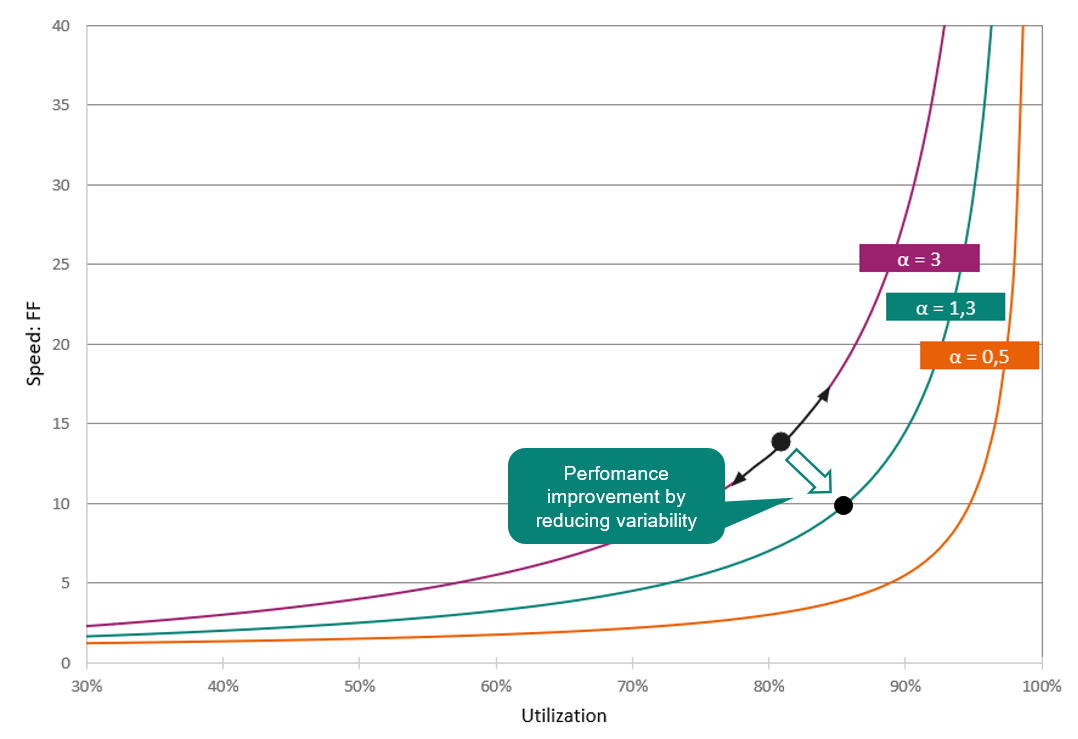
\includegraphics[width=0.7\textwidth]{Figures/OC.png}
    \caption{OC: By reducing variability ($\alpha$), the curve flattens out; with a low alpha, both U and speed can be improved simultaneously.}\label{fig:OC-fig}
\end{figure}
The OC's utility extends beyond merely understanding the TH-WIP relationship, it serves as both: a visualization- and decision-support tool in a range of operations (as stated in~\cite{LauterEhmReiner2025}).

Beyond day-to-day control, the OC provides a common language for operational and financial stakeholders. It enables consistent measurement of factory performance over time, comparison across lines or sites, benchmarking of future targets, and rapid what-if analysis when product mix, demand, or asset availability changes \citep{aurand1997operating}.\par
In summary, LCFM based on modeled processes and their execution as designed enables the implementation of lean strategies in complex flows by combining process stabilization, indicated by low alpha, with the operational control quantitative relationships of speed and U. Managers can forecast the effects of changes in WIP, mix, or U on TH and lead time, and make informed decisions on resource allocation, improvement sequencing, and cost optimization \citep{fayed2008, kalir2023optimizing}. The method emphasizes managing variability; reducing it steepens the OC \citep{hopp2001}, enabling higher TH for a given WIP and shorter CTs. Despite potential challenges in tailoring the method to non-manufacturing systems, we postulate that the same logic could be extended to other high-complexity domains that exhibit reentrant tasks, shared resources, and stochastic demand.     
            
    
\subsection{The 4 partners as components of the Operating Curve}\label{subsec:The 4 components of the Operating Curve}
Production capacity depends on the simultaneous availability of four foundational elements, termed the 4``M'' or 4 partners:
        \begin{itemize}
            \item HuMan (m1): operators and support personnel.
            \item Machine (m2): production equipment performing the operations.
            \item Material (m3): inputs such as lots, batches, and raw materials.
            \item Method (m4): the defined process and work instructions followed by human and machine.
        \end{itemize}
A production system operates only when all four elements are available simultaneously; the unavailability of any one element halts output. Capacity, therefore, depends on the overlap of their up-times. Aligning maintenance, staffing, material delivery, and changeover schedules to concentrate downtimes and maximize overlap of up-times increases productive time \citep{schoemig1999corrupting, ehm2011}.\\
Beyond the mean availability of each partner, poor synchronization of those and unpredictable schedule variability further reduce expected productive time and increase the need for buffers and slack capacity. Managing both availability and its variability is therefore essential for consistent, high-TH operations \citep{Schmielau2024}.


\subsection{Components of the Operating Curve needed for Non-Manufacturing Processes}\label{subsec:Components of the Operating Curve needed for Non-Manufacturing Processes}

Process modeling is fundamental to the application of OC principles, offering an end-to-end graphical representation of complex processes that facilitates the identification of improvement opportunities, including bottlenecks and integration gaps \citep{vanner2020bpmn}. BPMN offers a structured visualization of processes by delineating activities, roles, information flows, tools, and interactions, thereby fostering the shared understanding necessary for effective process-improvement analysis\citep{OMG2011}.

BPMN, however, yields a shared but essentially static graphical representation. To use the same models as a rigorous, reproducible basis for OC measurement, we formalize them into a machine-readable semantic layer based on OWL ontologies---an approach grounded in ontology-based business process management \citep{hepp2005semantic, thomas2009semantic} and in the semantic representation of manufacturing systems (Negri et al., 2016). This layer encodes the RPT of each unit process as a typed property and makes the resulting data queryable; it is instantiated for the analyzed cases in Section 5.

The OC characterizes the trade-off between U and cycle-time (CT) performance in a production line. U is defined in Eq.~(\ref{eq:U}), where TH and CapaP is the ideal capacity of the bottleneck resource, with 0 $<$ UT $<$ 1.\\ The FF is defined in Eq.~(\ref{eq:FF}) where CT is the total time a unit spends in the system, expressed in Eq.~(\ref{eq:CT_sum}) and Raw Processing Time (RPT) is the theoretical processing time deducted of waiting and QT represents the waiting time. The definition of the RPT involves decomposing unit processes into smaller, ideally elementary, tasks \citep{national1995unit}.
The execution time for each task is measured under ideal conditions to determine the minimum theoretical duration. The total RPT for the process is the sum of these individual times.\\
Little's Law, Eq.~(\ref{eq:WIP}), can be re-arranged as Eq.~(\ref{eq:TH}), showing how TH and WIP influence CT performance.\\
Finally, variability is given by the variability of the processing times and availabilities coming from the 4Ms\@. It is summarized by Eq.~(\ref{eq:alpha}).\par
Under the standard G/G/1 approximation, the OC can be expressed as Eq.~(\ref{eq:FF_OC})\@. This form implies that higher variability (larger $\alpha$) or higher UUM steepens the curve: small increases in U yield disproportionately large increases in FF and CT.


   \begin{table}[h!]
    \centering
    \caption{Equations used in OC key performance metrics.}
    \setlength{\tabcolsep}{12pt}   
    \renewcommand{\arraystretch}{2.2}
    \begin{tabular}{
        | >{\centering\arraybackslash}m{1.5cm}
        | >{\centering\arraybackslash}m{6cm}
        | >{\raggedright\arraybackslash}m{6cm} |
        }
        \hline
        \textbf{Eq.} & \textbf{Equation} & \textbf{Description}\\
        \hline
        % -------------------- 1 --------------------
        \refstepcounter{equation}\label{eq:U}
        (\theequation)
        &
        $\displaystyle U = \dfrac{TH}{\text{Capacity}}$
        &
        Utilization (U)
        \\
        \hline
        % -------------------- 2 --------------------
        \refstepcounter{equation}\label{eq:FF}
        (\theequation)
        &
        $\displaystyle FF = \dfrac{CT}{RPT}$
        & Flow Factor (FF)
        \\
        \hline

        % -------------------- 3 --------------------
        \refstepcounter{equation}\label{eq:CT_sum}
        (\theequation)
        &
        $\displaystyle CT = QT + RPT$
        & Cycle Time (CT) \\
        \hline
        % -------------------- 4 --------------------
        \refstepcounter{equation}\label{eq:WIP}
        (\theequation)
        &
        $\displaystyle WIP = CT \cdot TH $
        & Work-in-Progress (WIP) \\
        \hline
        % -------------------- 6 --------------------
        \refstepcounter{equation}\label{eq:TH}
        (\theequation)
        &
        $\displaystyle TH = \dfrac{WIP}{CT}$
        & Throughput (TH) (Little's Law)\\
        \hline
        % -------------------- 7 --------------------
        \refstepcounter{equation}\label{eq:alpha}
        (\theequation)
        &
        $\displaystyle \alpha = f(m_1,m_2,m_3,m_4) $
        & Variability ($\alpha$) \\
        \hline
        % -------------------- 8 --------------------
        \refstepcounter{equation}\label{eq:FF_OC}
        (\theequation)
        &
        $\displaystyle FF = 1 + \left(\dfrac{UT}{1-UT}\right)\alpha$
        & Operating Curve (OC) \\
        \hline
        
    \end{tabular}
\end{table}

%\vspace{0.5em}


In practice, bottlenecks are often costly or capacity-constrained resources, and departures from stationarity (e.g., time-varying arrivals or capacities) can invalidate steady-state relations; analyses should therefore be performed over stable operating periods.

When data indicate inefficiencies, the 8D methodology \citep{visser2017-8d} is implemented to stabilize processes and initiate improvements. The 8D reporting framework is a structured, eight-step approach that enables teams to investigate problems, identify and eliminate root causes, and develop long-term corrective actions. This method requires the active participation of relevant stakeholders, who collaborate concurrently to achieve effective and efficient (in form of a low alpha) problem resolution.
    



           
\subsection{Non-Manufacturing Processes in the Global Semiconductor Supply Chain}\label{subsec:Non-Manufacturing Processes in the Global Semiconductor Supply Chain}

As defined in previous research \citep{LauterEhmReiner2025}, our group of experts has created the definition ``non-manufacturing processes are activities within a semiconductor supply chain that do not directly add physical value to chips or wafers''. Wafer processing occurs in front-end (FE) fabrication facilities, whereas chip processing is conducted in back-end (BE) fabrication facilities. Non-manufacturing processes within global semiconductor supply chains can be categorized into three distinct areas:

a. Direct Supporting Process Flows: These encompass workflows associated with current semiconductor operations. These workflows are directly integrated into value-added process flows, such as the shipment of products between designated locations.

b. Indirect Supporting Process Flows: These pertain to the development and planning of new workflows required for novel semiconductor processes, including the creation of master data or auxiliary processes such as process analysis, which is not part of the primary manufacturing flow, or production planning.

c. Enabler Process Flows: These supporting functions facilitate the efficient operation of both existing and newly developed process flows, including administrative procedures or recruitment activities.

Recent studies and internal analyses indicate that a significant part of end-to-end lead-time variability arises from human-centric, information-driven workflows. The importance of these processes is further heightened by the VUCA inherent in the semiconductor industry, including short product life cycles, rapid technological advancements, globalized production networks, and fluctuating market conditions.

Although manufacturing processes have been systematically optimized using Factory Physics, LCFM, and OC management, the broader supply chain increasingly depends on administrative, planning, coordination, and governance activities. These activities exhibit substantially greater human-driven variability and fragmentation. Multiple studies demonstrate that flow inefficiencies, heuristic decision-making, unstable prioritization, and governance-driven changes \citep{Loesch2019,Kleinmuntz1987,Seddon2011} dominate the CTs of non-manufacturing workflows, frequently resulting in FFs that exceed manufacturing benchmarks.

The strategic implication is evident: as fabrication facilities approach theoretical OC optima, additional performance improvements for semiconductor companies will increasingly depend on stabilizing, synchronizing, and quantifying non-manufacturing workflows. Incorporating these processes into the same flow-oriented framework as manufacturing is essential for managing global semiconductor networks as a unified virtual fab environment \citep{ehm2011}, where both manufacturing and non-manufacturing activities are jointly optimized through consistent principles of variability management, flow efficiency, and end-to-end synchronization.

This perspective positions non-manufacturing processes as critical contributors to competitiveness, resilience, and responsiveness within the global semiconductor supply chain.



\subsection{Operating Curve in the Non-Manufacturing Context}\label{subsec:Operating Curve in the Non-Manufacturing Context}

As stated in the paper~\cite{LauterEhmReiner2025}, in non-manufacturing processes, the contribution of the 4M factors to variability is anticipated to change significantly. The human factor becomes increasingly dominant, whereas the machine component, often limited to the computer, becomes less relevant. The human element is expected to be the most influential factor.

\begin{figure}[h]
    \centering
    \includegraphics[width=1\textwidth]{Figures/4 Partner non manufacturing.png}
    \caption{\raggedright{}4 partners switching in non-manufacturing: this figure illustrates the anticipated transition within the four-partner methodology, which requires further evaluation.}\label{fig:operatingcurve}
\end{figure}

In non-manufacturing contexts, the approach to achieving efficiency shifts significantly due to the nature of variability. Unlike manufacturing, where variability often arises from machine states or technical CT fluctuations, non-manufacturing variability stems from human actions, decision-making behavior, and applied methods. Consequently, strategies designed for managing machine-driven variability must be adapted to human-centric workflows or replaced with approaches specifically suited to non-manufacturing environments. Principles from LCFM offer a valuable conceptual framework, emphasizing the stabilization of flow, reduction of unnecessary variability, and synchronization of work in complex, highly interdependent systems \citep{bauer2011LCFM,wikipediaCFP}.

Certain forms of variability in non-manufacturing processes can be reduced. Unverified or unvalidated workflows often contain avoidable inconsistencies that can be mitigated by clearer standards, improved information flow, or the deployment of higher-skilled personnel. Enhanced human availability, such as through ``follow-the-sun'' organizational structures, can decrease waiting times and improve end-to-end flow efficiency across global time zones.

However, some variability is inherent and cannot be fully eliminated, similar to manufacturing systems operating under high complexity. During periods of frequent process changes or governance-driven updates, non-manufacturing workflows may require strategies analogous to buffering and balancing used in production systems. In these situations, the optimal approach is not to suppress variability entirely, but to manage it deliberately through structured coordination mechanisms, flexible resource allocation, and targeted reduction of its impact on overall flow performance.

\section{Research Methodology}\label{sec:Research Methodology}

A quasi-experimental multi-case design \citep{Shadish2002} was employed to examine the applicability of OC principles and LCFM concepts to non-manufacturing enabling processes in global semiconductor supply chains. Two heterogeneous enabling workflows, Certificates of Employment request (CE) and New Hirings contract requests (NH), were selected as two intervention cases, complemented by the Costumer Requests for Product Specifications (CRPS) baseline case analysed in section 4. They exhibit sustained operational stability: although incremental adjustments have occurred over time, no structural breaks or disruptive transitions have been observed that would prevent the consistent application of a new analytic methodology \citep{rossini2019industry}.

Methodologically, this study is positioned as intervention-based research (IBR) as articulated by \citet{oliva2019intervention} and \citet{chandrasekaran2020ibr}, and building on the design-science tradition of \citet{vanaken2016design}. In IBR terms, a method ($M$) is used to apply a basket of theories ($T$) in order to move a problem situation ($S$) towards a desired state ($S^{*}$). Here, the theory basket $T$ comprises factory-physics-based OC management and LCFM; the method $M$ consists of BPMN-2.0 process modeling, FF/RPT measurement, 8D root-cause analysis, and iterative redesign; the situation $S$ is an inefficient, human-driven non-manufacturing workflow; and $S^{*}$ is a stabilized, synchronized flow with reduced FF\@. Crucially, IBR treats the intervention not only as a means of solving a field problem but as an instrument for theory development: where the intervention does not reach the expected $S^{*}$ (i.e., it ends in a surprising state $S'$), the resulting deviation triggers abductive reasoning that is used to recalibrate the theory basket $T$ --- in our case, the conjecture that factory physics requires a human-centric adaptation in non-manufacturing domains. This explicitly positions the present pretest--posttest design within an abductive research cycle (problem $\rightarrow$ theory $\rightleftarrows$ evidence $\rightarrow$ insight) rather than a purely deductive one.

Case 2, CE, was observed from February 2025 to December 2025, encompassing two redesign iterations with pre-post intervention samples (n=10) and a monthly process from July 2025 (n=33)\@. Use Case 3, NH, was tracked from November 2024 to December 2025, including two redesign cycles with pre-post intervention samples (n=25) and a monthly process between July and November 2025 (n=63). 

Data collection was conducted using a structured multistep procedure. Each process version was modeled with BPMN 2.0 \citep{OMG2011} to capture unit processes and decision points. These model established a consistent basis for deriving cycle-time components and calculating FF as the central efficiency metric, in accordance with established OC formulations \citep{hopp2001, fayed2008}. The RPT was measured as the optimal time without variability. Then, for each sample, CT was measured and aggregated into FF values. 

In addition, the BPMN models of the analyzed processes were formalized as OWL ontologies in Prot\'eg\'e \citep{musen2015protege} using Turtle syntax, attaching every measured RPT to its corresponding process element as a typed property. This semantic layer, detailed in Section 5, rendered the RPT values used in the FF computation reproducible and queryable via SPARQL \citep{harris2013sparql} rather than relying on manual extraction.

Each redesign was accompanied by an 8D root-cause analysis to systematically identify the influence of variability \citep{visser2017-8d}. The resulting interventions, aligned with core lean and LCFM principles, focused on (a) synchronization of the 4M partners, (b) digitalization of manual steps, and (c) standardization through reduction of process owners and simplification of approval logic. These three intervention types can be framed along the eight digital waste-reduction mechanisms of Lean~4.0 \citep{cifone2021lean40}: the digitalization and automation of manual steps operationalize the speed and precision mechanisms; the synchronization of the 4M partners, made transparent through the BPMN- and ontology-based representation of each workflow, reflects the visibility and feedback mechanisms; the standardization and simplification of approval logic enacts the prevention mechanism; and follow-the-sun staffing corresponds to the spatial and temporal flexibility mechanisms.

The analytical procedure comprised three distinct layers.
First, a within-case longitudinal analysis compared pre- and post-intervention \citep{Shadish2002} FF values and CT decompositions to assess the contribution of interventions to variability reduction. Second, a cross-case comparison \citep{Yin2018} identified common improvement mechanisms and contextual differences between the two workflows. Third, findings were interpreted in relation to OC behavior and lean management in manufacturing to evaluate structural differences in variability and flow. Descriptive statistics and pattern matching were employed to measure the results.

   
\section{Application of Non-Manufacturing Process on Lean for Complex Flow Manufacturing Enabler Processes}\label{sec:Application of Non-Manufacturing Process on Lean for Complex Flow Manufacturing Enabler Processes}

This chapter presents the application of OC-based analysis using FF measurements to identify opportunities for improvement in non-manufacturing workflows. The analysis is based on established LCFM, focusing on synchronization and variability reduction across the 4M. As discussed in Section~\ref{sec:Comparing Manufacturing and Non-Manufacturing Workflows}, the cases used are well-suited for examining the OC approach because they involve multiple operators who repeatedly participate in various steps of each process. Furthermore, the absence of ongoing changes in methods, process steps, or process ownership ensured process consistency across successive requests.

The initial case examines the FF within a non-manufacturing context, specifically focusing on the Customer Requests for Product Specifications
(CRPS) process. Unlike the subsequent cases, this analysis was conducted to establish empirical evidence of high FF values in a non-manufacturing workflow, thereby providing a baseline for later improvement-oriented applications. 

Customer Quality Management oversees the CRPS process, which begins when customers request changes to product specifications. This workflow engages
multiple teams, includes several approval and review activities, and requires extensive information exchange across departments. For systematic analysis, the process was modeled using BPMN~2.0 (see Figure~\ref{fig:crps}) and broken down into individual unit processes. RPT was established through process observations and expert assessments, while CT data were obtained from historical process records.

\begin{figure}[h]
    \centering
    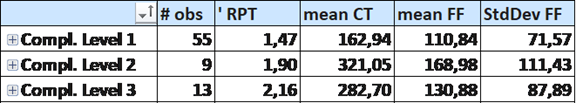
\includegraphics[width=0.9\textwidth]{Figures/CRPS.png}
    \caption[width=0.9\textwidth]{\raggedright{}CRPS flow factor versus request complexity: higher request complexity does not translate proportionally into higher FF; waiting times and coordination losses dominate the observed FF values, which exceed typical manufacturing benchmarks.}\label{fig:crps}
\end{figure}

The analysis revealed a substantial difference between the direct processing effort required to complete a request and the overall lead time experienced by the process. While the actual work content remained relatively limited, requests spent significant time waiting between process steps, approvals, and handovers. The results indicate that increasing request complexity does not necessarily lead to proportional increases in FF (see Figure~\ref{fig:crps bpmn}). Instead, process performance is strongly influenced by waiting times and coordination losses that contribute more strongly to overall performance than direct processing effort. However, the calculated FF values were considerably higher than those typically observed in manufacturing environments. These findings confirm that high FF values are characteristic of many non-manufacturing processes, in which coordination activities, prioritization decisions, and information flows contribute substantially to total cycle time.

\begin{figure}[h]
    \centering
    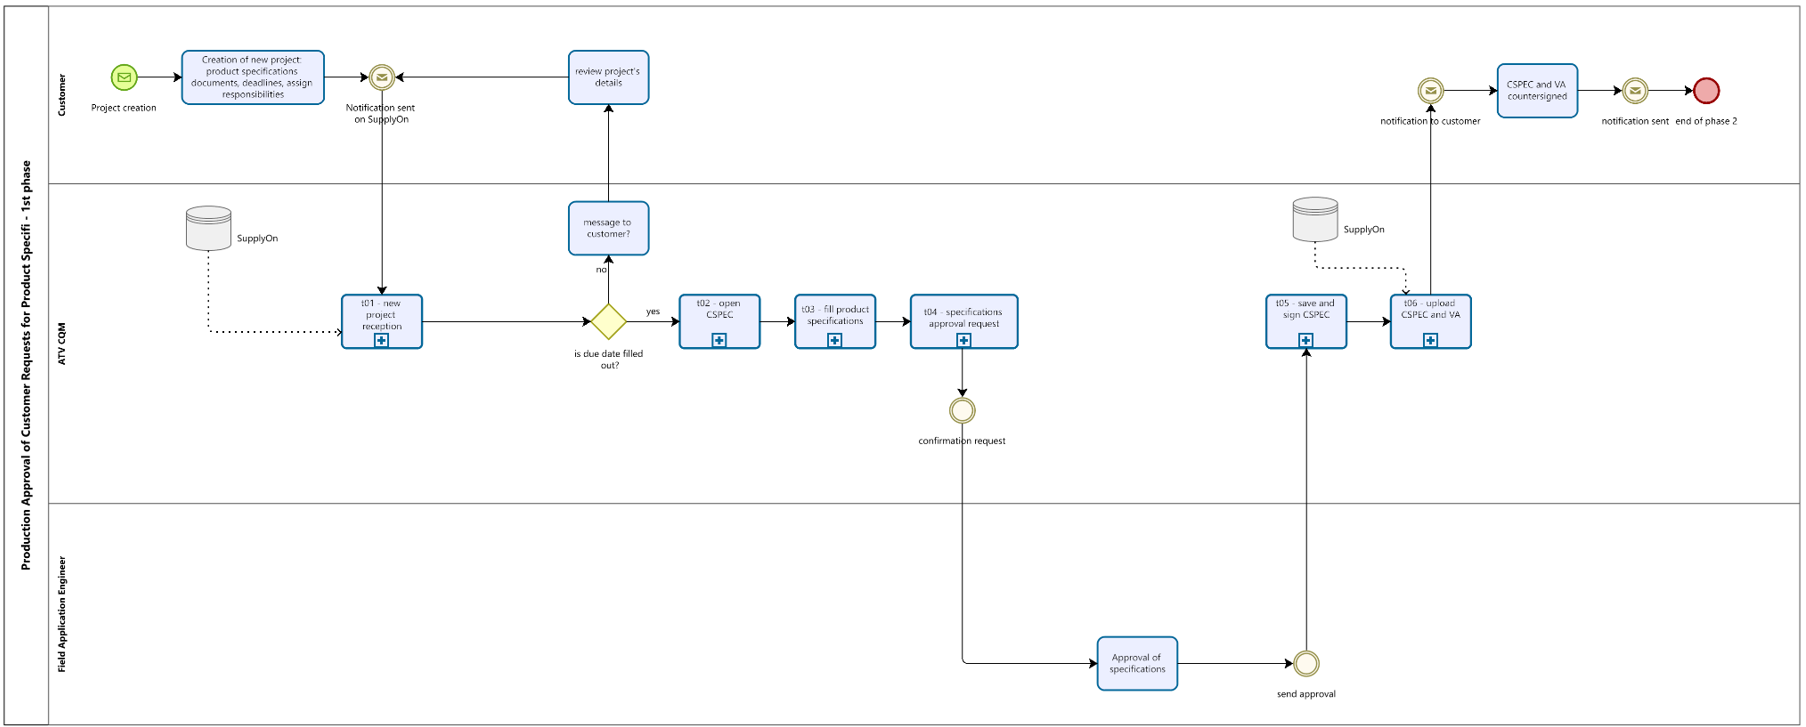
\includegraphics[width=0.9\textwidth]{Figures/CRPS BPMN.png}
    \caption[width=0.9\textwidth]{\raggedright{}CRPS unit process BPMN 2.0 visualization: the figure shows the process flow of the CRPS process used to establish the non-manufacturing FF baseline.}\label{fig:crps bpmn}
\end{figure}

This first case demonstrates the suitability of FF as a metric for identifying improvement potential in human-centric workflows. Although no intervention was conducted within the CRPS process, the analysis provided empirical evidence for the existence of high FF values in non-manufacturing environments. This finding motivated the subsequent application of the OC-based methodology to new processes, where targeted interventions were implemented to reduce variability, improve synchronization, and ultimately enhance process performance.

The second case investigates the creation of certificates of employment (CE), a human-centered administrative workflow that generates formal employment documentation. To ensure accurate process representation and quantification of RPT, all unit steps were modeled using BPMN 2.0. Therefore, the process was decomposed into smaller unit processes and assigned an RPT based on time measurements collected as an operator completed a request under controlled conditions.

\begin{figure}[h]
    \centering
    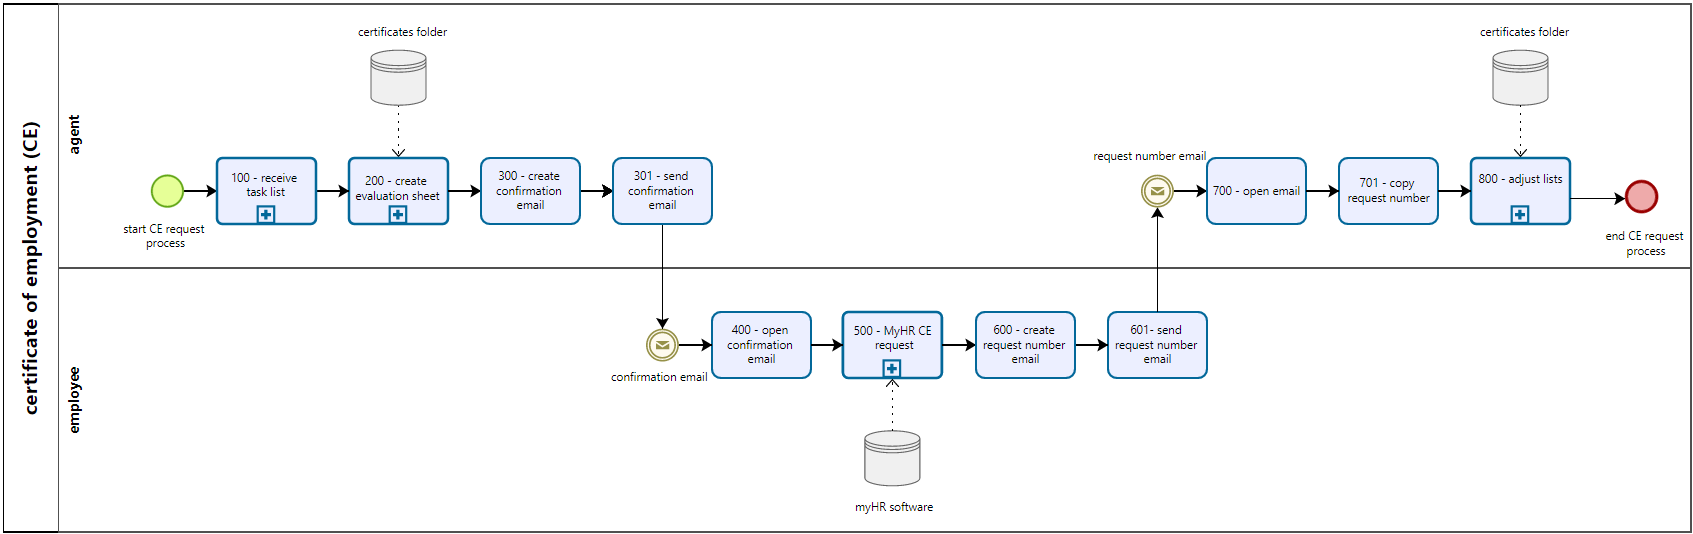
\includegraphics[width=0.9\textwidth]{Figures/CE_BPMN.png}
    \caption[width=0.9\textwidth]{\raggedright{}CE unit process BPMN visualization \citep{niklasifx2023CE}: the figure shows the process flow of the used CE unit processes.}\label{fig:CE_BPMN}
\end{figure}

The third case analyzes the new contract request hiring process (NH), which involves initiating an employment contract within the organization. This workflow encompasses the formulation of job requirements, sequential approvals by internal stakeholders, and the formal creation of the contract document. The same steps as in the first case were followed to document the process and define the RPT\@.

\begin{figure}[h]
    \centering
    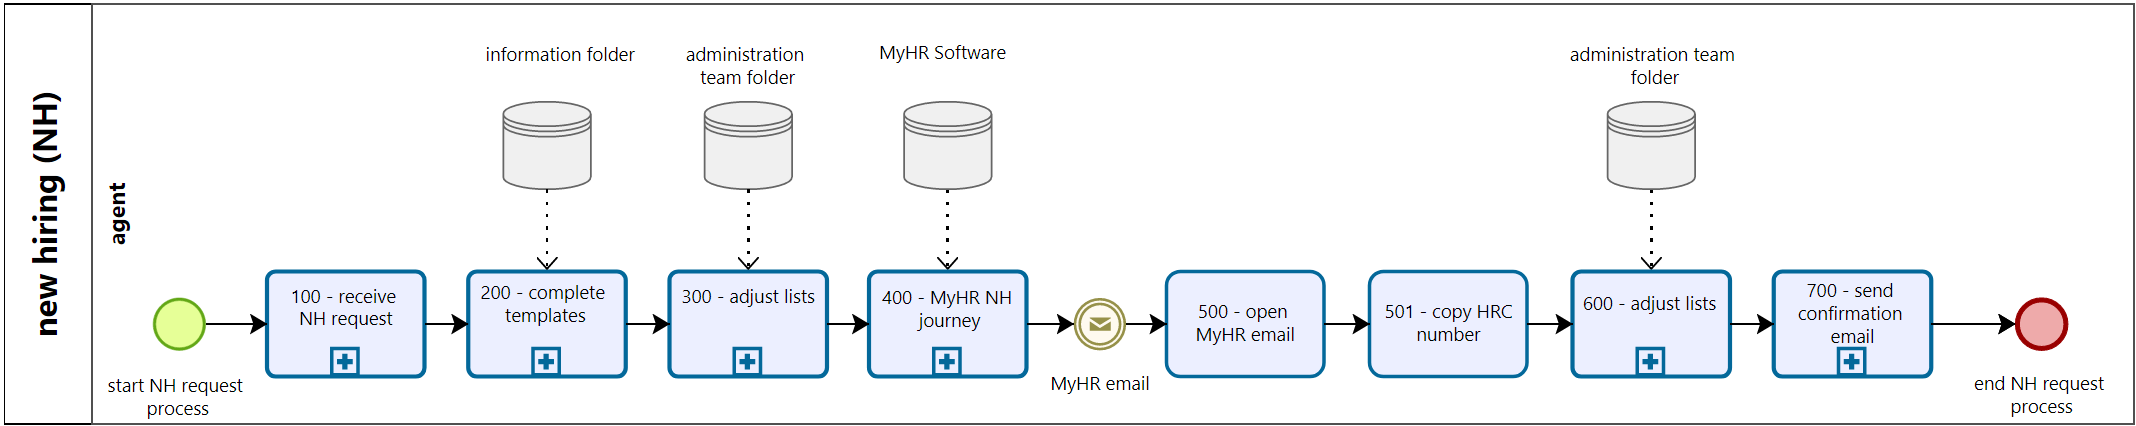
\includegraphics[width=0.9\textwidth]{Figures/NH_BPMN.png}
    \caption{\raggedright{}NH unit processes BPMN visualization \citep{niklasifx2023NH}: the figure shows the process flow of the used NH unit processes.}\label{fig:NH_BPMN}
\end{figure}

Across both intervention cases (CE and NH), the findings demonstrate substantial improvements over previous processes.\\
In CE, the results demonstrate the development of the FF following the major intervention to fully digitalize the request process. Additional measures, including the automation of email templates, further reduced the RPT by a factor of nearly two. Consequently, the FF appears higher in the current process (see Fig.~\ref{CE-old-new} and~\ref{fig:ff-rpt-ff}). Further synchronization and improvement of the adjusted process is necessary to achieve more stable and improved long-term performance. %add part that i told you on webex!

    \begin{figure}[!htb]
    \centering
        \begin{subfigure}{0.34\textwidth}
        \centering
        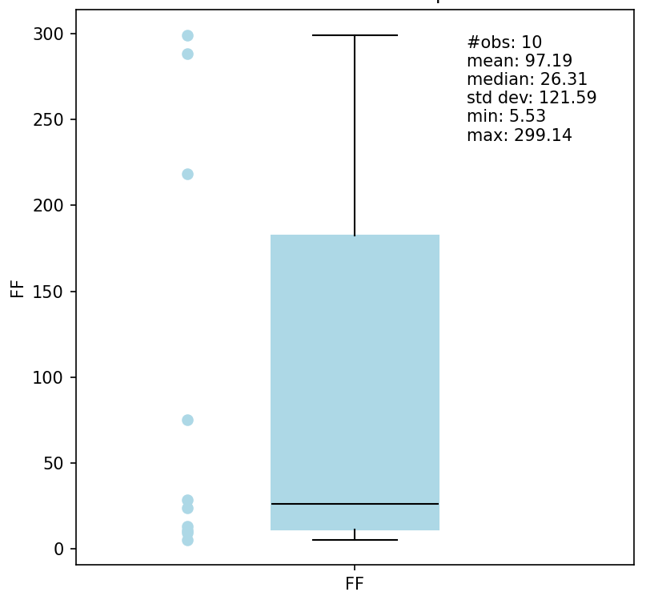
\includegraphics[width=\linewidth]{Figures/FF-certificates-old.png}
        \caption{old CE process: the figure illustrates the previous certificate process prior to the implementation of additional interventions. This version reflects the most recent changes following interventions, which can be viewed at~\cite{LauterEhmReiner2025}. A smaller part of the process than in the previous work was implemented.}\label{fig:FFCertificates_old process}
        \end{subfigure}
        \hfill
    \begin{subfigure}{0.62\textwidth}
        \centering
        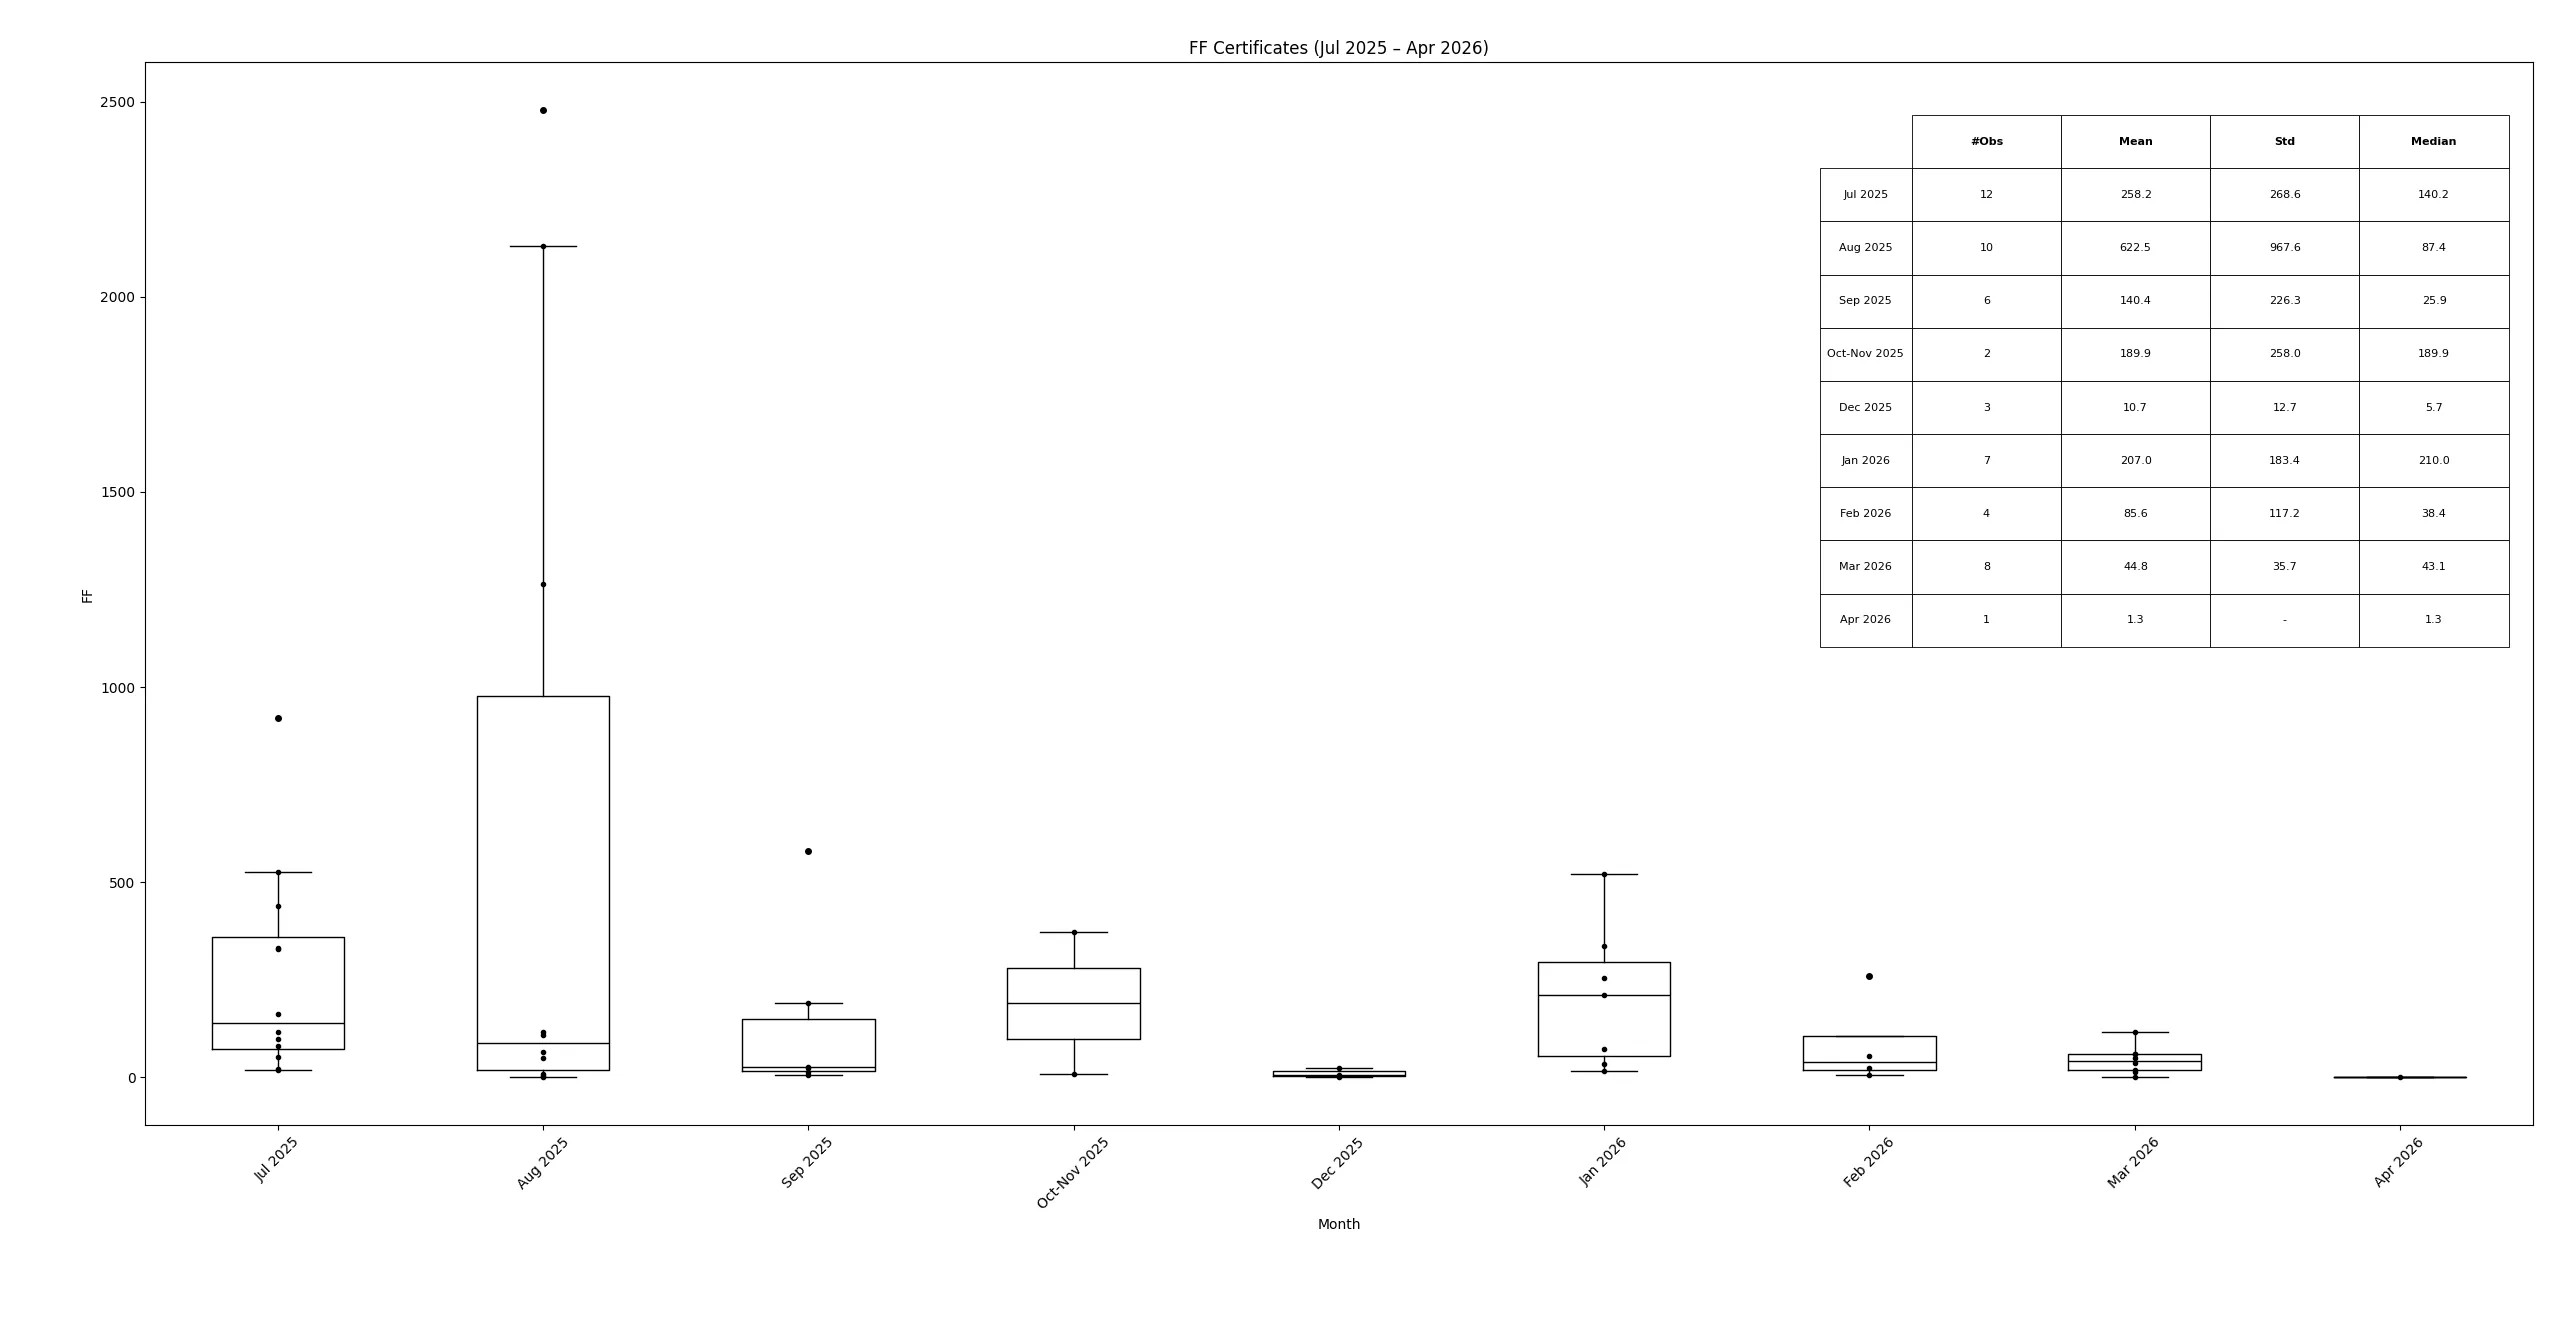
\includegraphics[width=\linewidth]{Figures/3. BoxPlots_Certificates.jpg}
        \caption{reporting CE boxplots from July 2025 to April 2026: the figure shows the samples (n=33), mean (reaching from 10.67 to 603.99), median (5.68 to 186.82) and standard deviation (reaching from 12.69 to 979.11) for the different months. It shows an increase of the three statistical measures in the month of August.}\label{fig:coe-box}
        \end{subfigure}
        \caption{CE old and current process}\label{CE-old-new}
    \end{figure}
    
    \begin{figure}[h]
        \centering
        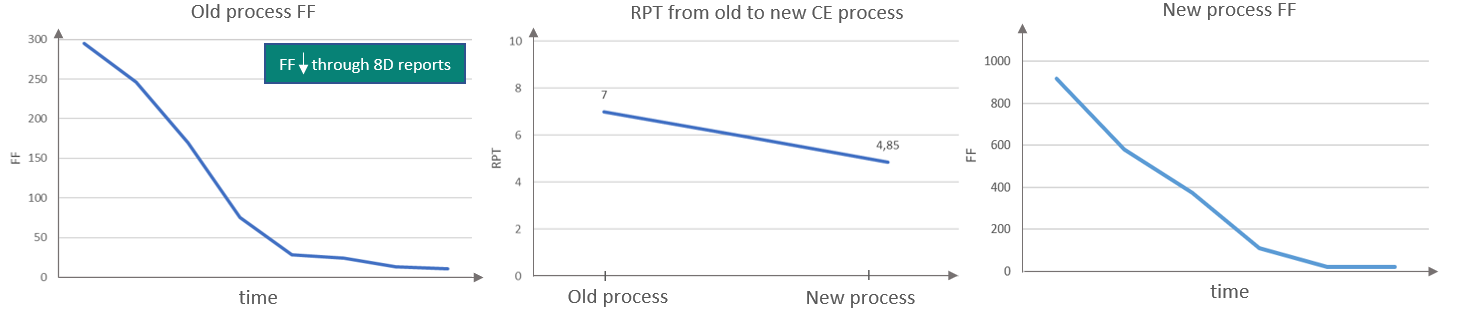
\includegraphics[width=\textwidth]{Figures/ff-rpt-ff-graph.png}
        \caption{FF improvement through 8D reporting, automation of tasks reduce the RPT from 7 to 4.85, FF increases.}\label{fig:ff-rpt-ff}
    \end{figure}

    \begin{figure}[!htb]
        \centering
        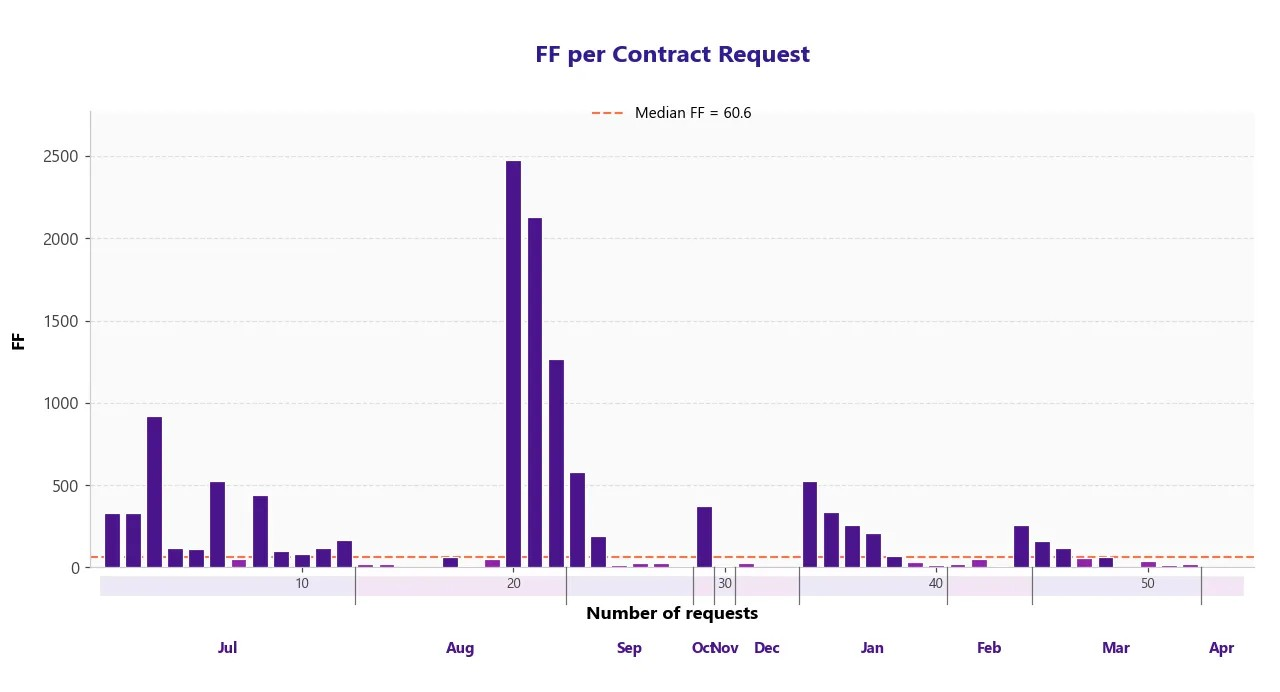
\includegraphics[width=0.99\textwidth]{Figures/1. BarChart_Certificates.jpg}
        \caption{\raggedright{}evolution of certificate FF from July 2025 to April 2026: a total of 33 samples were analyzed (as seen on the x-axis). The results show the variability in the process environment, visible in the different peaks.
        }\label{fig:FFCertificates_July-Dec}
    \end{figure}

The deviating data in August (see Fig.~\ref{CE-old-new} and~\ref{fig:FFCertificates_July-Dec}) were investigated using 8D reporting, which attributed them to the human operator's holiday period. Additional peaks are associated with insufficient task synchronization, elevated workload, and inconsistent prioritization. The CE process changed compared to previous research in~\cite{LauterEhmReiner2025}: a part of the process moved to another process owner, the RPT went down, the CT changed, and therefore the FF changed. This adjustment was done to make the old process date comparable to the current reported one (see Fig.~\ref{fig:coe-box}).

    \begin{figure}[!htb]
    \centering
        \begin{subfigure}{0.34\textwidth}
        \centering
        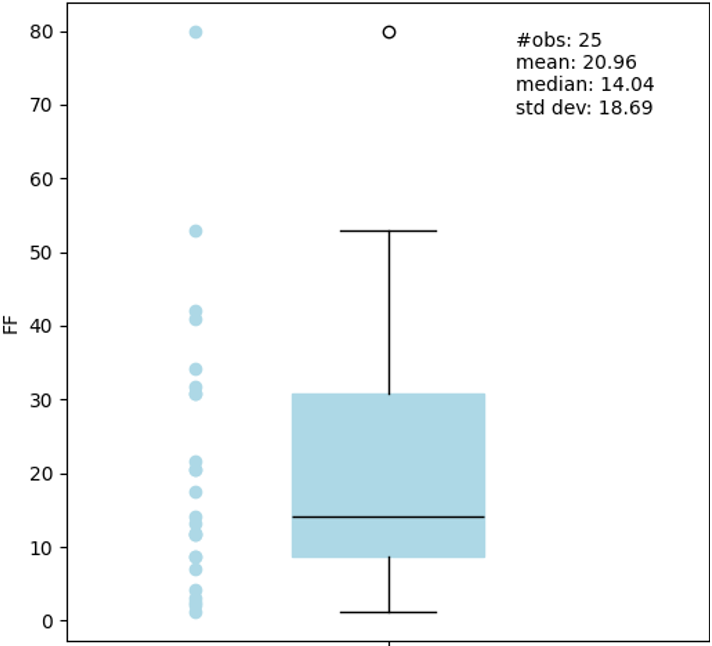
\includegraphics[width=\linewidth]{Figures/FFContracts_old process.png}
        \caption{old NH process: the figure illustrates the previous NH process prior to the implementation of additional interventions. This version reflects the most recent changes following interventions, which can be viewed at~\cite{LauterEhmReiner2025}. A small change in the RPT led to a slightly adjusted graph in this paper.}\label{fig:FFContracts_old process}
        \end{subfigure}
        \hfill
        \begin{subfigure}{0.62\textwidth}
        \centering
        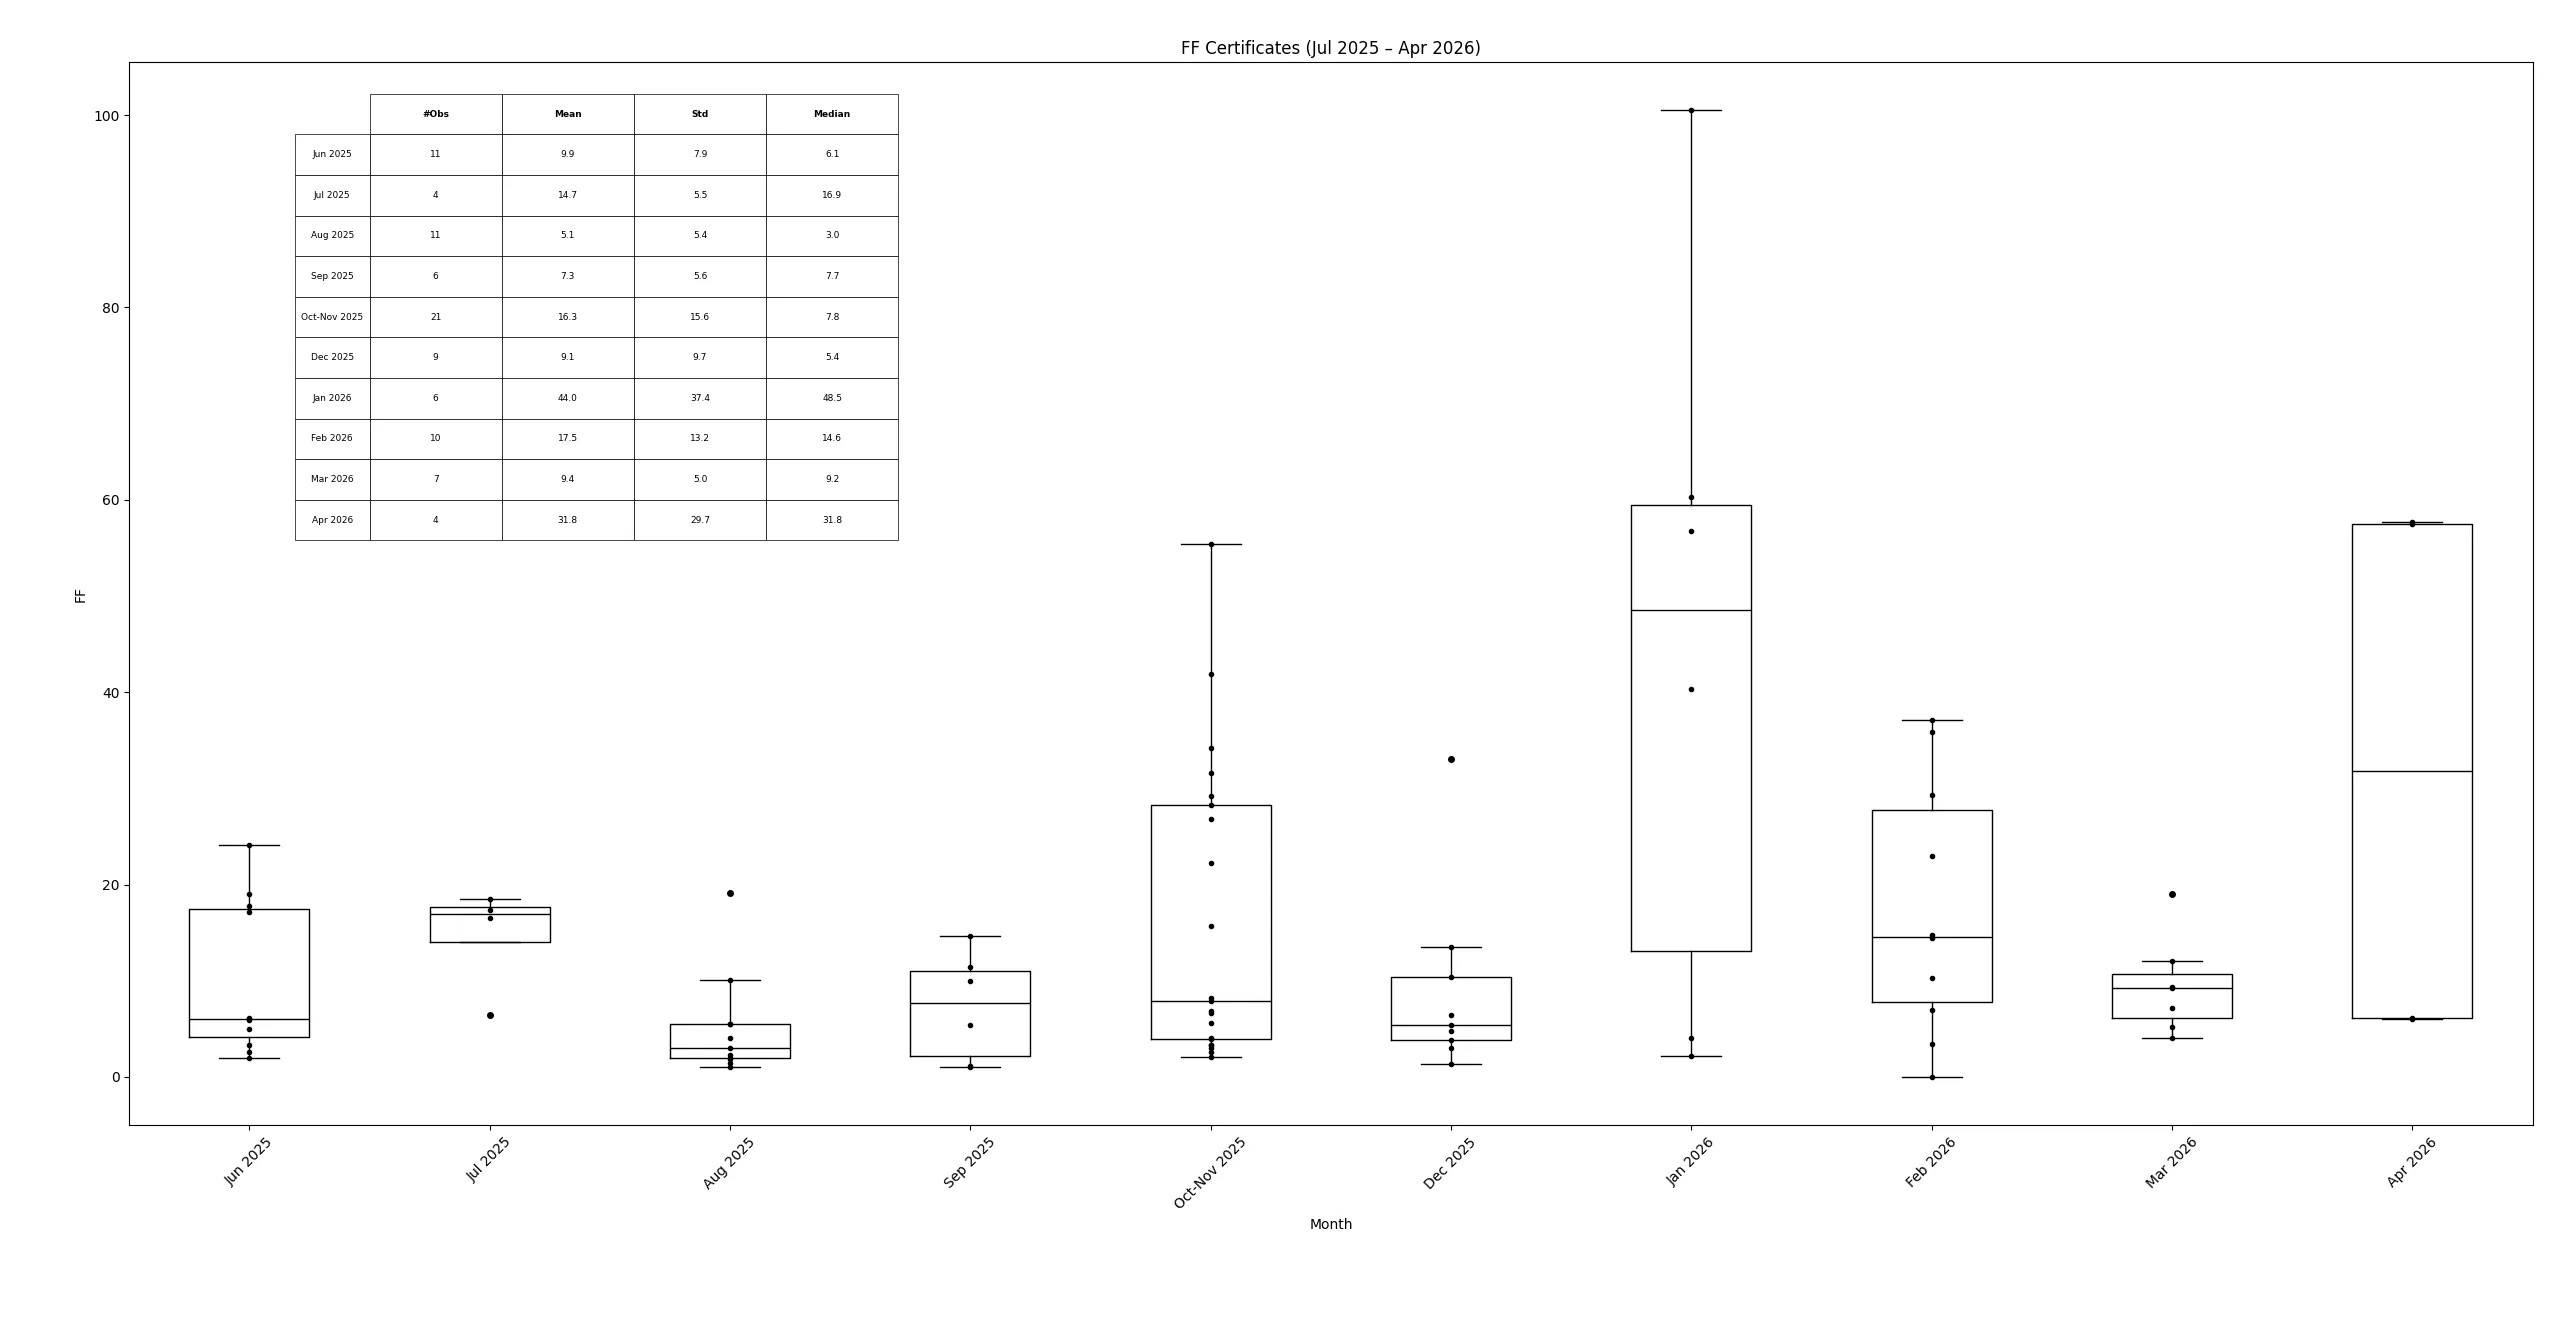
\includegraphics[width=\linewidth]{Figures/4. BoxPlots_Contracts.jpg}
        \caption{reporting NH boxplots from June 2025 to April 2026: the figure shows the samples (n=63), mean (reaching from 5.09 to 21.52), median (from 2.98 to 18.21) and standard deviation (reaching from 5.35 to 19.16) for the different months. It shows an increase of the three statistical measures in the months of October and November.\\}\label{fig:contracts-box}
        \end{subfigure}
        \caption{NH old and current process}\label{fig:NH-old-new}
    \end{figure}

In NH, the comparison with the previous process reveals an improvement in process stability following renewed synchronization among all partners (see Fig.~\ref{fig:NH-old-new}). The FF remains relatively stable throughout the observed months, with deviations attributable to the operator's absence in October (see Fig.~\ref{fig:contracts-box} and~\ref{fig:FFContracts_June-Dec}, as documented in the 8D report) and increased workload at the end of November.

\begin{figure}[!htb]
    \centering
    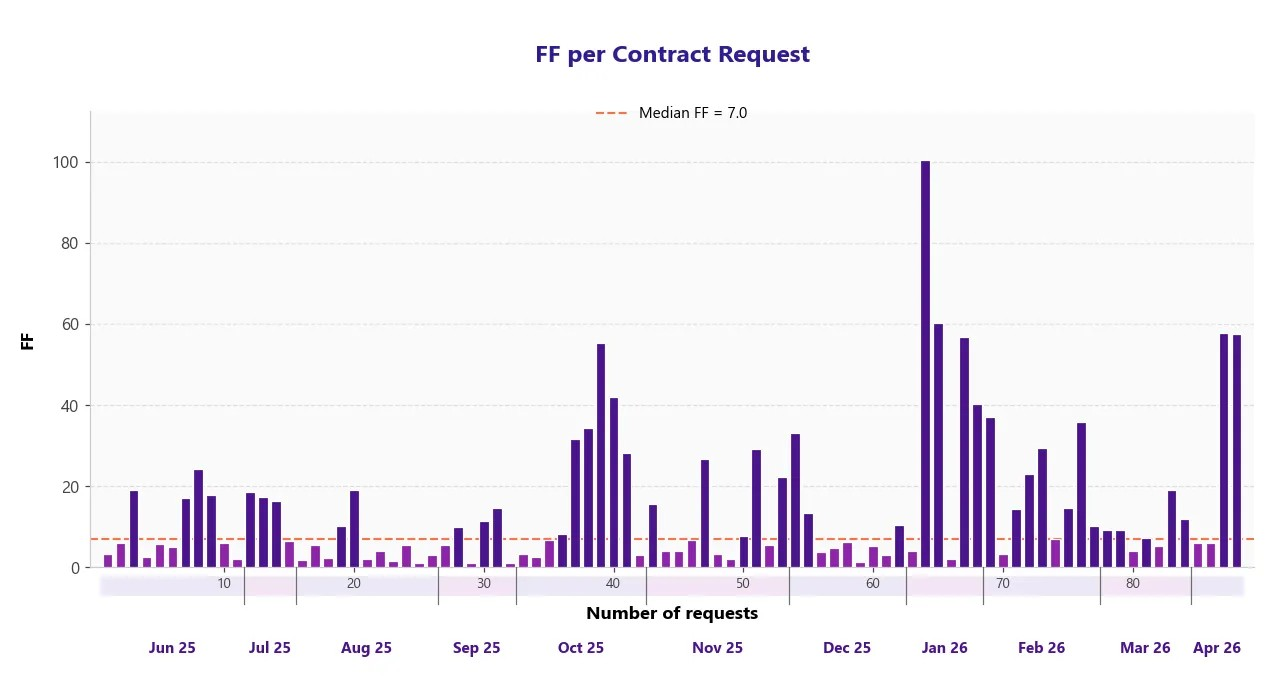
\includegraphics[width=\textwidth]{Figures/2. BarChart_Contracts.jpg}
    \caption{\raggedright{}evolution of NH FF from June to December 2025: a total of 63 samples were analyzed (as seen on the x-axis). The results show the variability in the process environment, visible in the different peaks. 
    }\label{fig:FFContracts_June-Dec}
\end{figure}

The active identification of value streams using BPMN2.0 and 8D reporting has contributed to reduced RPT, as demonstrated in CE through the automation of certain operator tasks, resulting in measurable quantitative improvement in both cases. 

While the resulting FF values may not align with standard manufacturing benchmarks, typically ranging from 2 to 4, the relative improvement from the initial state \citep{LauterEhmReiner2025} represents a significant achievement.

Interpreted through the intervention-based-research lens established in Section~\ref{sec:Research Methodology}, these results carry significance beyond their immediate quantitative gains. Although the deployed OC theory basket measurably reduced both RPT and FF in the CE and NH workflows, the resulting operating points did not converge towards the manufacturing-typical FF corridor of $2$ to $4$ that a purely deductive transfer of factory physics would anticipate. The residual variability that prevented this convergence proved to be predominantly governance-driven and tied to cross-functional handoffs, fluctuating prioritisation, and the limited availability of the human partner, rather than to machine states or technical processing-time fluctuations. In IBR terms, this systematic deviation between the desired state ($S^{*}$) and the empirically observed state ($S'$) constitutes an anomaly that cannot be accounted for within the original theory basket. Consistent with the abductive logic underlying this study, the anomaly is therefore treated not as a failed transfer of factory-floor logic but as a warrant for theory refinement: it motivates the inference that, within the 4M model, the human partner ($m_{1}$) constitutes the dominant and only partially reducible source of variability in non-manufacturing workflows. This recalibration of the underlying theory---the human-centric adaptation of factory physics---is developed in Section~\ref{sec:Conclusion and Future Work}.


\section{From BPMN Models to a Queryable Semantic Layer}
5.1 Ontology Design and Construction
To extend the analysis of the BPMN-based process models described earlier, two of the unit processes examined in this study — the New Hiring (NH) contract request and the Certificate of Employment (CoE) request — were formalized as OWL ontologies. Both processes are executed by the same organizational role (Student Admin 1) and were therefore selected as an initial example for semantic formalization within the LCFM framework.
The ontology layer serves three purposes. First, it establishes a shared vocabulary across the four LCFM partners: Human, Machine, Material, and Method. Second, it provides a machine-readable model between every observed task duration and its corresponding BPMN element, directly encoding the raw process time (RPT) of each unit process. Third, it supports cross-case comparability between the NH and CoE workflows under a unified semantic framework, facilitating Operating Curve benchmarking across processes.
The models were built in Protégé using Turtle syntax and adhere to the OWL 2 framework [1]. Core BPMN 2.0 elements were declared as named OWL classes: UserTask, StartEvent, IntermediateEvent, EndEvent, SequenceFlow, Role, and DataStores. All object-property domains and ranges were explicitly restricted to enforce semantic consistency.
Each process step and sub-step is instantiated as a named individual carrying the following assertions: triggeredBy, hasSequenceFlow, hasSubProcess, isPerformedBy, and usesDataStore as object properties. Empirically measured task durations, originally recorded in MM:SS format, are attached to each individual via the hasDurationMinutes datatype property. Both ontologies are publicly available via Zenodo [2], with interactive visualizations and full source files accessible via the links provided in the figure captions below.

5.2 Ontology Visualization 
 
Figure 1 – New Hiring Ontology in WebVOWL
Figure 1 shows the WebVOWL [3] visualization of the New Hiring ontology. Nodes represent OWL classes — including UserTask, StartEvent, IntermediateEvent, EndEvent, SequenceFlow, Role, and DataStores — along with their named subclasses corresponding to process steps 100 through 700 and sub-steps 201 through 502. Directed edges represent object properties such as triggeredBy, hasSequenceFlow, hasSubProcess, isPerformedBy, and usesDataStore, as well as the datatype property hasDurationMinutes, which carries the empirically measured RPT of each step in decimal minutes. Interactive visualization: https://service.tib.eu/webvowl/#iri=https://raw.githubusercontent.com/cobrie23tcd/OWL-Ontology-of-Unit-Processes-/main/NewContractsOntology.ttl

 
Figure 2 – Certificate of Employment Ontology in WebVOWL
Figure 2 presents the equivalent visualization for the Certificate of Employment ontology. The same node and edge conventions apply as in Figure 1. Interactive visualization: https://service.tib.eu/webvowl/#iri=https://raw.githubusercontent.com/cobrie23tcd/OWL-Ontology-of-Unit-Processes-/main/CertificatesOfEmploymentOntology.ttl. 
Full source files: https://github.com/cobrie23tcd/OWL-Ontology-of-Unit-Processes-

5.3 SPARQL for Data Querying
SPARQL (SPARQL Protocol and RDF Query Language) [4] is the W3C-standardized query language for RDF-based knowledge graphs and enables structured retrieval of typed data from an ontology without requiring manual extraction. SPARQL queries can retrieve, for example, the cumulative RPT of all sub-tasks within a composite step, the data stores accessed by a given role, or the full precedence chain between two events. This capacity to extract structured data on demand distinguishes a semantic knowledge graph from a conventional BPMN model and enables the ontology to function as an analytical instrument.
To execute the queries presented below, each ontology was loaded into Apache Jena Fuseki [5], an open-source SPARQL server. Fuseki allows one or more named graphs — in this case, unit process ontologies — to be hosted simultaneously within a single dataset. 
This architecture is scalable: as additional unit process ontologies are populated with RPT and cycle time data and loaded into the same Fuseki dataset, the query interface provides process data retrieval across all unit processes, forming the foundation for a unified non-manufacturing knowledge graph. 
The examples below illustrate query patterns applied to the loaded datasets:
SPARQL Example 1

SPARQL Example 2

SPARQL Example 3

SPARQL Example 4



\section{Conclusion and Future Work}\label{sec:Conclusion and Future Work}

The application of OC management principles, as well as Lean and LCFM, to non-manu-facturing workflows in the global semiconductor supply chain demonstrates that LCFM as well as OC can systematically improve flow efficiency in human-driven enabling processes. Standardization and digitalization reduced variability and reduced the FF\@. Monthly reports revealed that human variability remains the primary driver of performance. A mix of OC management, lean value stream tracking, digitalization, and automization enabled reducing the FF in CE and NH compared to previous process versions (see~\cite{LauterEhmReiner2025}), keeping them stable at a lower average. This shows the potential of those principles in the non-manufacturing environment.

Interpreted through the lens of intervention-based research, the central contribution is not merely the confirmed FF reduction but the abductive insight produced by the interventions. The OC theory basket was a plausible starting point, yet deploying it in human-in-the-loop workflows consistently surfaced a surprise: a large share of the residual variability is governance-driven and stems from cross-functional handoffs, and the achieved FF values do not reach the manufacturing benchmark range of 2--4. This deviation between the expected and the observed outcome is exactly the trigger that, in IBR, warrants a recalibration of the theory: factory physics does not transfer unchanged to non-manufacturing domains but requires a human-centric adaptation in which the human partner of the 4M model carries the dominant, only partially reducible, source of variability. Framing the study this way turns an apparent limitation into its main theoretical result.

The analysis indicates that human-driven variability cannot be fully eliminated, making deliberate balancing strategies essential. This finding underscores the need for more robust synchronization among the four partners (see~\ref{subsec:The 4 components of the Operating Curve}). It also suggests that follow-the-sun staffing models could mitigate variability by increasing temporal flexibility across global time zones. 

Building on the semantic layer introduced in Section~5, future work will extend the ontology-based representation to additional non-manufacturing unit processes, enabling SPARQL-driven, cross-process Operating Curve benchmarking on a unified knowledge graph and a systematic, machine-readable capture of the human-centric variability identified above. Based on that, the future requires an agent-based simulation that can run through different stages of the process.

As supply chains grow in complexity, extending LCFM principles to non-manufacturing workflows opens new efficiency opportunities, enabling management of global semiconductor supply chains as one ``virtual fab'' \citep{ehm2011}.





\bibliographystyle{elsarticle-harv} 
\bibliography{Yourbibfile}

    %% else use the following coding to input the bibitems directly in the
    %% TeX file.
    
    %\begin{thebibliography}{00}
    %\begin{thebibliography}{00}
    
    %% \bibitem[Author(year)]{label}
    %% Text of bibliographic item
    
    %\bibitem[ ()]{}
    
    %\end{thebibliography}

\newpage
\section*{ }\label{sec:Author short Biography}

    \noindent \textbf{Niklas Lauter} is pursuing a Ph.D.\ in Production Management at Vienna University of Economics, Austria. He holds a B.A.\ in Social Science and an M.A.\ in Sociology. His email address is \href{mailto:niklas.lauter@infineon.com}{niklas.lauter@infineon.com}.
    
    \vspace{1em} 
    \noindent \textbf{Silvia Casati} is pursuing a M.Sc.\ Degree in Industrial Management Engineering at Politecnico di Milano, Italy. She is conducting her Master Thesis at Infineon Technologies AG\@. Her email address is \href{mailto:nsilvia.casati@infineon.com}{silvia.casati@infineon.com}.
    
    \vspace{1em} 
    \noindent \textbf{Hans Ehm} is a Senior Principal Engineer in Supply Chain and heads the Supply Chain Innovation department at Infineon Technologies AG\@. He holds a diploma in Applied Physics from HS Munich and an M.S.\ in Mechanical Engineering from Oregon State University. His email address is \href{mailto:hans.ehm@infineon.com}{hans.ehm@infineon.com}.
    
    \vspace{1em} 
    \noindent \textbf{Gerald Reiner} is a professor in the field of Operations Management. He holds a diploma in Business Administration and has completed his doctorate and habilitation with a focus on optimizing operations and supply chain processes. His academic and professional expertise lies in areas such as sustainable supply chains, production planning, and integrating digital technologies into traditional business processes. His email address is \href{mailto:gerald.reiner@wu.ac.at}{gerald.reiner@wu.ac.at}.\\

\end{document} 
